\documentclass[10pt,a4paper]{article}
\usepackage[margin=1.85cm]{geometry}
\usepackage[T1]{fontenc}
\usepackage[utf8]{inputenc}
\usepackage{lmodern,microtype}
\usepackage{amsmath,amssymb,booktabs,graphicx,xcolor,hyperref,url}
\usepackage{enumitem,fancyhdr,caption,subcaption,tabularx,float,cite,array}
\definecolor{deepblue}{HTML}{04364A}
\definecolor{teal}{HTML}{176B87}
\hypersetup{colorlinks=true,linkcolor=deepblue,citecolor=teal,urlcolor=teal,
 pdfauthor={Tom Graci},pdftitle={Taxonomy-Aware Ensembling for Multi-Taxa Acoustic Recognition in the Pantanal}}
\pagestyle{fancy}\fancyhf{}
\lhead{BirdCLEF+ 2026 -- Multi-taxa acoustic recognition}
\rhead{Tom Graci}\cfoot{\thepage}\setlength{\headheight}{14pt}
\setlist[itemize]{leftmargin=*,topsep=3pt,itemsep=2pt}
\captionsetup{font=small,labelfont=bf}
\newcolumntype{Y}{>{\raggedright\arraybackslash}X}

\title{\vspace{-1.2cm}\textcolor{deepblue}{\textbf{Taxonomy-Aware Ensembling of Perch Sequence Models and Distilled Sound Event Detectors}}\\[3pt]
\Large Multi-Taxa Acoustic Recognition in the Pantanal for BirdCLEF+ 2026}
\author{\textbf{Tom Graci}\\Independent Researcher\\
ORCID: \href{https://orcid.org/0009-0000-0448-4012}{0009-0000-0448-4012}\\
\href{https://github.com/gtom-pandas/birdclef-2026-research}{github.com/gtom-pandas/birdclef-2026-research}}
\date{July 21, 2026}

\begin{document}
\maketitle

\begin{abstract}
BirdCLEF+ 2026 required multi-label recognition of 234 animal taxa in five-second windows of passive acoustic monitoring data from Brazil's Pantanal, under an offline 90-minute CPU inference constraint. This paper presents an evidence-audited competition system that combines two public solution families: a Perch-v2 representation pipeline with prototype and state-space sequence heads, and a distilled convolutional sound-event-detection (SED) pipeline. The private-best submission used a direct 3:97 mixture of two attributed public notebook outputs, followed by sequential genus- and class-level probability smoothing. It achieved public/private macro ROC-AUC values of 0.95035/\textbf{0.94216}; the account finished \textbf{947th of 4,094 teams}. Beyond reporting the score, we reconstruct the complete active inference graph, explain why each component addresses a challenge-specific failure mode, and compare it with the official write-ups of the first-, second-, third- and fifth-place solutions. The comparison identifies a shared 2026 recipe: short in-domain windows, Perch transfer or distillation, SED CNNs, soundscape pseudo-labels, deliberately diverse ensembles, taxon specialists and conservative temporal or ecological post-processing. The study's contribution is reproducible integration, provenance recovery, experiment selection and critical synthesis; it does not claim authorship of the upstream Perch, ProtoSSM, ResidualSSM or distilled SED architectures. Because no controlled ablation was preserved, leaderboard differences are treated as observational rather than causal.
\end{abstract}

\noindent\textbf{Keywords:} bioacoustics, passive acoustic monitoring, BirdCLEF, Perch v2, sound event detection, state-space models, knowledge distillation, taxonomy-aware ensemble.

\section{Introduction}
Passive acoustic monitoring (PAM) can survey wildlife continuously across sites and seasons, but automated recognition in tropical soundscapes is not a conventional single-label audio problem. Several animals may vocalise simultaneously; foreground calls may occupy only a fraction of a five-second interval; microphones record wind, insects and anthropogenic noise; and the curated focal recordings used for training differ substantially from autonomous-recorder soundscapes. BirdCLEF+ 2026 placed these issues in the Pantanal and expanded the target set beyond birds to amphibians, insects, mammals and one reptile \cite{kahl2026birdclef}.

The competition metric was macro ROC-AUC over evaluable classes. This gives rare and common taxa equal class-level weight, while making probability calibration less important than correct within-class ranking. The execution environment added another constraint: inference had to run offline on CPU within 90 minutes. A competitive design therefore needed strong transfer features, economical temporal modelling and complementary predictors rather than a single large end-to-end network.

This paper answers four questions. First, what did the private-best submitted notebook actually execute? Second, why are its Perch, sequence, SED and taxonomy components technically relevant to this challenge? Third, how does that design compare with the approaches reported by leading participants? Fourth, what conclusions are justified by the preserved evidence, and what would require a new experiment?

The contributions are:
\begin{itemize}
  \item a metadata-backed analysis of the 234-class task and its long tail;
  \item a reconstruction of the active prediction graph, including upstream authorship and notebook-version identifiers;
  \item a technical account of the prototype/state-space heads, SED branch, fusion gates and taxonomy smoothing;
  \item a comparative synthesis of official top-team write-ups and relevant primary literature;
  \item a reproducibility release containing the canonical notebook, asset manifest, extracted training code, deterministic final blending code and tests.
\end{itemize}

\section{Task, data and challenge-specific failure modes}
\subsection{Formal task}
For each soundscape file split into $T$ non-overlapping five-second windows, the system predicts $P\in[0,1]^{T\times C}$, where $C=234$. A row may contain several positive taxa. Macro ROC-AUC averages the class-wise AUC over classes having both positive and negative examples in the evaluated set. The objective therefore rewards robust ranking for every taxon and is especially sensitive to neglecting rare target groups.

\subsection{Verified exploratory analysis}
The official \texttt{train.csv} contains 35,549 focal recordings; \texttt{taxonomy.csv} defines 234 targets. Only 206 targets occur as primary labels and 28 never occur as a primary label. Among the observed primary classes, counts range from 1 to 499 recordings, with a median of 125. Exactly 4,372 rows (12.30\%) list at least one secondary label. The metadata do not contain audio duration, so this paper does not invent a duration distribution.

\begin{table}[H]
\centering
\caption{Statistics computed directly from the official metadata.}
\begin{tabular}{lr}\toprule
Property & Value\\\midrule
Focal training recordings & 35,549\\
Competition targets & 234\\
Targets observed as primary labels & 206\\
Targets absent as primary labels & 28\\
Rows with secondary labels & 4,372 (12.30\%)\\
Recordings per observed primary class & min 1; median 125; max 499\\
Taxonomic composition & 162 Aves; 72 non-avian\\
Prediction granularity & 5 seconds\\\bottomrule
\end{tabular}
\end{table}

\begin{figure}[H]
\centering
\begin{subfigure}{0.54\textwidth}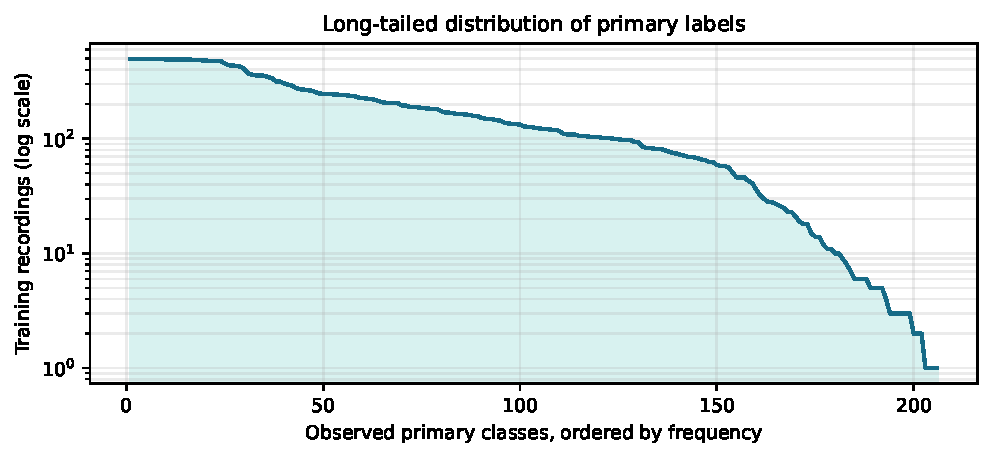
\includegraphics[width=\linewidth]{figures/class_frequency.pdf}\caption{Primary-label long tail.}\end{subfigure}\hfill
\begin{subfigure}{0.43\textwidth}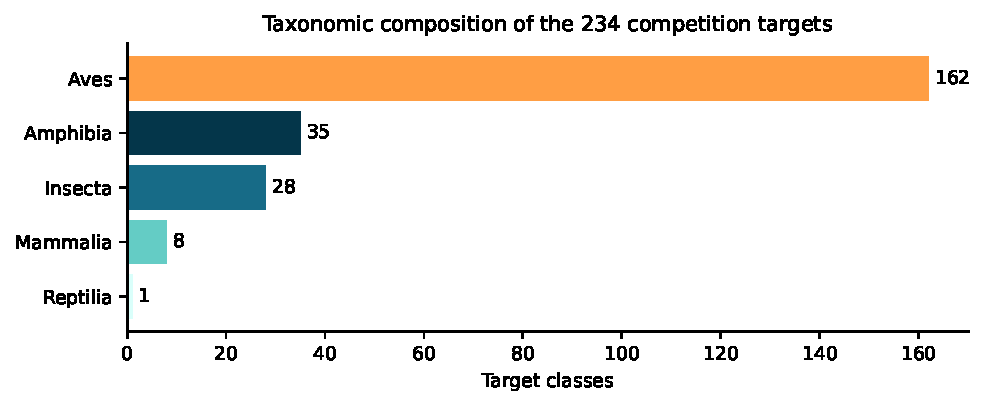
\includegraphics[width=\linewidth]{figures/taxonomy.pdf}\caption{Target taxonomy.}\end{subfigure}
\caption{Evidence-backed EDA. Non-avian targets comprise 35 Amphibia, 28 Insecta, 8 Mammalia and 1 Reptilia classes.}
\end{figure}

\subsection{Why this task needs more than a classifier}
Four coupled shifts shape the solution. \emph{Label shift}: the focal table is severely long-tailed and omits 28 targets as primary labels. \emph{Acoustic-domain shift}: focal recordings often centre a labelled organism, whereas PAM audio is polyphonic and background-dominated. \emph{context shift}: site and hour alter the plausible taxon distribution. \emph{taxonomic shift}: a foundation model's output vocabulary does not perfectly coincide with the competition taxonomy. These shifts motivate transfer embeddings and prototypes for low-data classes, in-domain SED models for soundscape structure, priors for ecological plausibility, and ensembles for errors that are not perfectly correlated.

\section{Technical background}
\subsection{Perch transfer representations}
Perch embeddings were trained at large scale for bioacoustic transfer and can support new classifiers with limited labelled data \cite{ghani2023perch}. Perch 2.0 broadens the pretraining domain through self-distillation and prototype learning across animal taxa \cite{vanmerrienboer2025perch2}. In this challenge they serve two distinct roles: direct taxon evidence from mapped output logits, and a 1,536-dimensional representation on which small competition-specific heads can be trained. The latter is attractive under a CPU limit because the expensive encoder is frozen and the learned heads are compact.

\subsection{Sound-event detection with spectrogram CNNs}
An SED network converts a waveform into a time--frequency representation and predicts class activity over time. EfficientNet-family backbones provide a strong accuracy/compute trade-off through compound scaling \cite{tan2019efficientnet}. Unlike a clip-level prototype head, an attention or framewise SED head is designed to preserve local events. This is useful when a short call is embedded in a noisy five-second mixture. SpecAugment, waveform mixup and frequency-response perturbation are common means of improving robustness \cite{park2019specaugment,zhang2018mixup}.

\subsection{Distillation, pseudo-labels and sequence modelling}
Knowledge distillation transfers a teacher's soft structure into a smaller or differently parameterised student \cite{hinton2015distilling}. Noisy Student extends this idea by repeatedly using teacher predictions on unlabelled examples while training a perturbed student \cite{xie2020noisystudent}. For BirdCLEF, unlabelled soundscapes are particularly valuable because they represent the target acoustic domain, but incorrect pseudo-labels can reinforce site-specific errors.

Structured state-space models (SSMs) offer a recurrent formulation with efficient long-sequence processing \cite{gu2021s4}. Audio adaptations show the relevance of bidirectional state-space processing for acoustic representations \cite{zhang2024audiomamba}. The reproduced sequence heads here use SSM-like selective recurrences over the twelve five-second windows of a one-minute soundscape, allowing adjacent evidence to influence a window without applying a heavy transformer to raw spectrograms.

\section{What leading BirdCLEF+ 2026 teams explored}
Official participant write-ups reveal convergence on a family of solutions rather than one dominant architecture. Table~\ref{tab:landscape} summarises only author-reported methods; scores and improvements are not assumed transferable to the present system.

\begin{table}[H]
\centering\small
\caption{Solution landscape from official BirdCLEF+ 2026 write-ups. KD: knowledge distillation; PL: pseudo-labels.}
\label{tab:landscape}
\begin{tabularx}{\textwidth}{p{1.0cm}YYY}\toprule
Rank & Core models & Training/domain adaptation & Diversity and post-processing\\\midrule
1st \cite{first2026writeup} & SED- and MLP-head CNNs, Perch-v2 linear head, Amphibia/Insecta and genus specialists & Perch embedding distillation followed by full fine-tuning; iterative Noisy Student; competition focal and soundscape data & Diverse heads, label spaces and inputs; rank blending; five-second chunks\\
2nd \cite{second2026writeup} & Perch public branch, EfficientNet-v2-S/B0, NFNet, SED branch, Insecta specialist & Five rounds of PL; focal and soundscape data; some XC-pretrained backbones; BCE or soft-AUC+BCE & Near-equal ensemble; model correlation considered; 87-minute CPU inference\\
3rd \cite{third2026writeup} & EfficientNet-v2-S SED and SEResNeXt26 Perch-KD models & Fixed sampling shares for focal/labeled/unlabelled soundscapes; one PL round; rare-class and site-aware sampling & Feature/backbone diversity; TTA; site/hour priors; file confidence and temporal smoothing\\
5th \cite{fifth2026writeup} & HGNetV2-B0, EfficientNetV2-S/B3, Perch prototype and SED branches & Perch distillation, self-distillation and PL; focal plus labelled soundscapes; mixup and SpecAugment & Dual-window TTA, neighbour smoothing, peak scaling; weighted CNN/prototype/SED ensemble\\
This work & Public Perch--ProtoSSM--ResidualSSM and distilled SED integration & Lightweight heads trained on cached Perch features; public attached checkpoints/caches & Rank-aware internal fusion; 3:97 top blend; genus then class smoothing\\\bottomrule
\end{tabularx}
\end{table}

The first-place solution explicitly used two phases: cosine embedding distillation from Perch v2, then full fine-tuning and multi-iteration Noisy Student training. Its reported example progressed from 0.935 supervised to 0.946, 0.950 and 0.949 over three pseudo-label rounds, illustrating both the value and eventual saturation of self-training \cite{first2026writeup}. It also found five-second chunks more effective than longer inputs and used specialist output spaces to preserve non-bird and genus-level performance.

The second-place author deliberately kept some models free of Perch distillation because distillation improved single models but increased their correlation. Their final system mixed Perch, an SED-derived EfficientNet, several pseudo-label rounds and an Insecta specialist; the overall public/private scores were reported as 0.959/0.960 despite substantial movement in individual branches \cite{second2026writeup}. This is a useful caution: a stronger individual model is not automatically a better ensemble member.

The third-place system offers the closest independent confirmation of several operations found inside the reproduced Model\_51: five-second 32-kHz inputs, Perch KD, EfficientNet SED, shifted-window TTA, site/hour priors, file confidence scaling, rank-aware scaling and adaptive temporal smoothing \cite{third2026writeup}. The fifth-place solution likewise reported complementary prototype and SED branches and incremental benefits from distillation, pseudo-labels, TTA and post-processing, though its numeric deltas are specific to that author's pipeline \cite{fifth2026writeup}.

A separate 2026 study compared frozen Perch token representations with a supervised HGNetV2-B0 SED backbone and a non-bird prototype head, reporting private 0.936 and rank 1,894 \cite{miyaguchi2026tokens}. This supports the broader research question behind the competition: whether pretrained acoustic tokens can match or complement supervised spectrogram CNNs. The evidence from the top write-ups favours complementarity rather than replacement.

\section{Reconstructed system architecture}
\subsection{Provenance and reference submission}
The authenticated submission archive contains 79 submissions, 50 with retained score rows. Submission reference 53075232, informally named ``EoS.8'' in the notebook history, is the private-best result at 0.95035 public and 0.94216 private. The name is retained only as an audit identifier; it is not used as a scientific method name.

The top-level notebook consumed two full prediction matrices (Table~\ref{tab:provenance}). Model\_22 is yukiZ's reproduction of a Perch+ProtoSSM+ResidualSSM pipeline. Model\_51 is Derek's EoS.4/rank-power notebook and contains an extensive Perch/SED ensemble. This paper describes their active code because it determined the submitted result, while explicitly crediting the upstream authors.

\begin{table}[H]
\centering
\caption{Active top-level inputs and provenance.}
\label{tab:provenance}
\begin{tabularx}{\textwidth}{lYlr}\toprule
Input & Public source & Function & Weight\\\midrule
Model\_22 & yukiZ, \emph{Bird26 REPRODUCE Perch+ProtoSSM+ResSSM}, Kaggle version 309368265 \cite{yukiz2026model22} & independent sequence-pipeline prediction & 0.03\\
Model\_51 & Derek, \emph{BirdCLEF 2026 exp019 EoS4 rank power 06}, Kaggle version 320064228 \cite{derek2026model51} & Perch/SED ensemble prediction & 0.97\\\bottomrule
\end{tabularx}
\end{table}

\begin{figure}[H]\centering
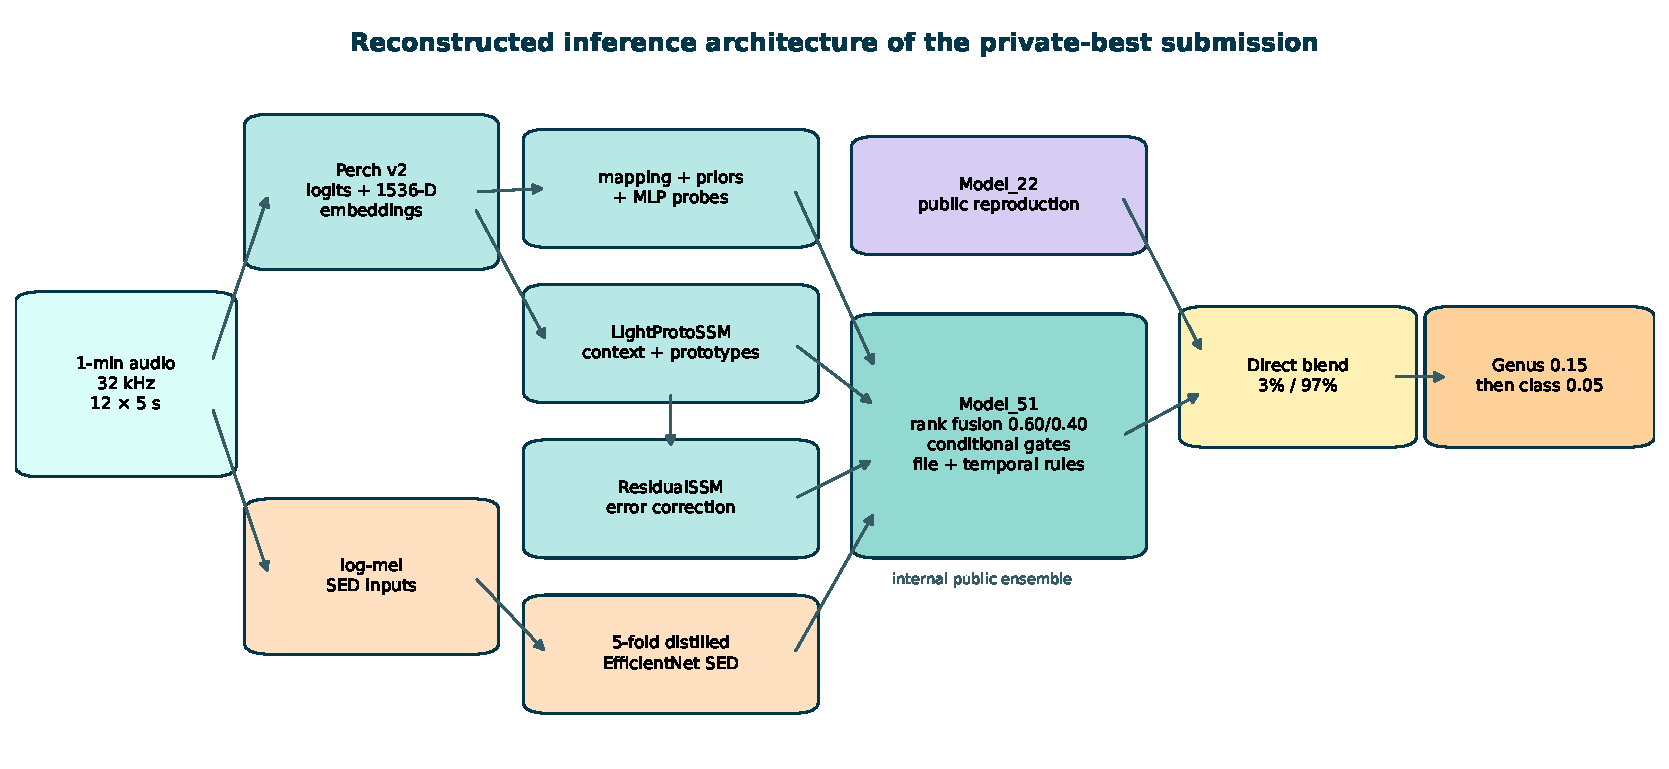
\includegraphics[width=0.98\textwidth]{figures/architecture.pdf}
\caption{Reconstructed active prediction graph. Solid arrows are executed prediction flow; the final 3:97 blend and taxonomy smoothing are reproduced exactly in \texttt{src/infer.py}.}
\label{fig:architecture}
\end{figure}

\subsection{Audio segmentation and Perch evidence}
Each one-minute soundscape is resampled to 32 kHz and divided into twelve five-second windows. Perch v2 produces a 1,536-dimensional embedding $e_t$ and source-vocabulary logits for each window $t$. A taxonomic mapping transfers compatible source labels to competition targets. Mapped classes receive direct evidence; unmapped or weakly mapped targets rely more heavily on learned prototypes, ecological priors and the SED branch. Model\_51's first-pass code assigns different mapped/unmapped weights (0.60 and 0.35 respectively), which is a pragmatic response to vocabulary mismatch rather than a learned calibration.

Temporal test-time augmentation shifts the one-minute sequence by $\{0,1,-1,2,-2\}$ windows and also evaluates a reversed sequence. The transformations do not create new acoustic content; they test sensitivity of the sequence head to boundary placement and direction. Averaging reduces variance at the cost of additional lightweight-head inference, while the Perch embeddings themselves remain cached.

\subsection{LightProtoSSM head}
LightProtoSSM projects $e_t\in\mathbb{R}^{1536}$ to $d=128$, adds positional information and embeds site and hour metadata. Two bidirectional selective-SSM blocks process the twelve-window sequence, with a multi-head attention interaction. A simplified selective recurrence for channel state $h_t$ is
\begin{align}
\Delta_t &= \operatorname{softplus}(W_\Delta x_t), \qquad A=-\exp(A_{\log}),\\
h_t &= h_{t-1}\odot \exp(A\Delta_t) + (B_t\odot x_t)\Delta_t,\\
y_t &= \langle C_t,h_t\rangle + D\odot x_t.
\end{align}
The reverse-time branch is flipped back and fused with the forward branch. This context model is technically appropriate because a call near a window boundary may be clearer in an adjacent window, and continuous soundscapes exhibit short-range persistence. It is not intended to model seasonal ecology across files.

Class prototypes $q_c$ are constructed from training embeddings. Cosine similarity produces a temperature-scaled logit
\begin{equation}
z^{\mathrm{proto}}_{tc}=\tau\frac{u_t^\top q_c}{\|u_t\|\,\|q_c\|}.
\end{equation}
The network fuses prototype evidence with mapped Perch logits. Prototypes are helpful for few-shot targets because they require estimating a class centre rather than a full deep classifier, but a poor centre can be fragile under call-type or recorder shift.

The extracted training stage uses full-batch AdamW, a capped positive-class weight, BCE-with-logits and a logit-distillation term:
\begin{equation}
\mathcal{L}=\mathcal{L}_{\mathrm{BCE}}(z,y)+0.15\,\|z-z^{\mathrm{teacher}}\|_2^2.
\end{equation}
The executed defaults are 40 epochs, learning rate $10^{-3}$ and patience 8. The distillation term anchors the small head to pretrained evidence while allowing correction from competition labels.

\subsection{Ecological priors and MLP probes}
Model\_51 builds smoothed priors from labelled soundscapes for site, hour and their interaction. In general form, a sparse bucket estimate is shrunk toward the global rate:
\begin{equation}
\tilde\pi_{c,b}=\frac{N_b}{N_b+K}\hat\pi_{c,b}+\frac{K}{N_b+K}\hat\pi_c.
\end{equation}
The prior modifies model evidence rather than replacing it. This can disambiguate acoustically similar taxa with different habitat or diel activity, but it risks encoding survey bias. Therefore priors should remain weak and be evaluated on held-out sites.

Small MLP probes operate on reduced Perch features and provide additional nonlinear class boundaries. Their value is primarily diversity: a probe trained directly on embeddings makes different errors from mapped logits and a temporally contextualised prototype head. The notebook combines these signals before the residual stage; the repository does not claim that every internal weight is an independently validated optimum.

\subsection{ResidualSSM correction}
ResidualSSM receives the Perch embedding and first-pass logits, processes them with a smaller bidirectional SSM and learns residual targets
\begin{equation}
r_{tc}=y_{tc}-\sigma(z^{(1)}_{tc}), \qquad
p^{(2)}_{tc}=\operatorname{clip}\!\left(\sigma(z^{(1)}_{tc})+\hat r_{tc},0,1\right).
\end{equation}
Residual learning focuses capacity on systematic first-pass errors rather than relearning the complete classifier. The executed defaults are 30 epochs, learning rate $10^{-3}$ and patience 8, with a deterministic 15\% file-level validation split. Splitting by file prevents windows from the same recording appearing in both partitions, although it is not a substitute for geographic validation.

\subsection{Distilled SED branch and conditional fusion}
The complementary branch uses five distilled EfficientNet SED folds exported to ONNX. Spectrogram CNN features capture local time--frequency patterns that Perch prototypes may miss, especially for sonotypes or non-bird taxa. Model\_51 first combines prototype and SED predictions through rank-aware blending (0.60 prototype, 0.40 SED) and then applies conservative conditional gates. Examples visible in the canonical code include suppressing prototype-only spikes when $p_{\mathrm{proto}}>0.5$ but $p_{\mathrm{SED}}<0.05$, restoring temporally continuous prototype evidence when contextual rank is high, and admitting strong SED-only evidence when the SED rank is extreme. These gates encode disagreement patterns, not biological laws.

For soundscape-only sonotypes and rare Amphibia, Mammalia and Reptilia targets, the notebook includes specialised mirroring or threshold logic. Such rules address classes poorly represented by focal primary labels, but they are among the most leaderboard-sensitive components and require explicit class-wise validation before ecological deployment.

\subsection{File-level and temporal post-processing}
The internal Model\_51 path applies file confidence scaling, rank-power adjustment and adaptive local smoothing. If $m_c=\max_t p_{tc}$, rank-power scaling increases separation using an exponent of 0.65. Adaptive smoothing moves an uncertain window toward neighbouring evidence while retaining confident peaks. This matches the metric's emphasis on within-class ordering and the physical continuity of acoustic events. However, excessive smoothing can smear a brief call into adjacent windows and create false positives, so the coefficient is kept small.

\subsection{Score-defining top-level blend}
After row/column alignment, the private-best notebook computes
\begin{equation}
P^{(0)}=0.03P^{22}+0.97P^{51}.
\end{equation}
The 3\% Model\_22 contribution is best interpreted as a low-risk diversity injection into the stronger Model\_51 prediction, not as a balanced ensemble. The preserved archive contains the submitted result but no clean 0/100 versus 3/97 controlled comparison; a causal gain cannot be assigned to the 3\% component.

\subsection{Sequential taxonomy smoothing}
For each multi-member scientific genus $g$,
\begin{equation}
\bar P_{ig}=|g|^{-1}\sum_{c\in g}P^{(0)}_{ic},\qquad
P^{(g)}_{ic}=0.85P^{(0)}_{ic}+0.15\bar P_{ig}.
\end{equation}
Then, for each multi-member taxonomic class $k$,
\begin{equation}
P^{\mathrm{final}}_{ic}=0.95P^{(g)}_{ic}+0.05\bar P^{(g)}_{ik}.
\end{equation}
Genus precedes class. The rationale is that related taxa may share acoustic morphology or habitat and that a strong sibling prediction can weakly regularise an uncertain class. The risk is equally concrete: congeners can be acoustically distinct or mutually exclusive, and class-level averaging across Aves is biologically coarse. The small coefficients limit, but do not eliminate, this risk. No isolated scored ablation was preserved, so taxonomy smoothing is reported as an executed operation, not a demonstrated improvement.

\section{Experimental trajectory and official result}
\begin{table}[H]
\centering
\caption{Selected official submission milestones. These are successive systems, not controlled single-factor ablations.}
\begin{tabularx}{\textwidth}{lYrr}\toprule
Date & Submission label & Public & Private\\\midrule
Apr 20 & Version 3 LightGBM & 0.92948 & 0.92345\\
May 1 & ProtoSSM + EfficientNet & 0.93515 & 0.93640\\
May 2 & ONNX Perch sequence + SED & 0.94307 & 0.93793\\
May 18 & EoS.5 & 0.94903 & 0.94075\\
May 27 & private-best reference submission & 0.95035 & \textbf{0.94216}\\
Jun 3 & final selected submission & \textbf{0.95087} & 0.94138\\\bottomrule
\end{tabularx}
\end{table}

\begin{figure}[H]\centering
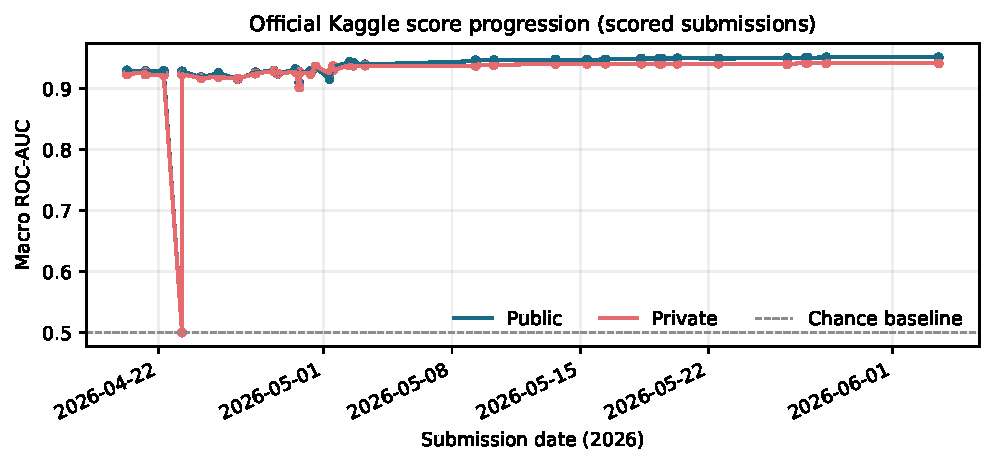
\includegraphics[width=0.90\textwidth]{figures/score_progression.pdf}
\caption{Official public/private score history for retained scored submissions. The isolated 0.5 result is a degenerate submission retained for auditability.}
\end{figure}

The completed leaderboard lists team \emph{T Soo} (Kaggle user \texttt{ttgrcgrc}) at rank 947 of 4,094, the top 23.1\%. The final selected submission increased public score by 0.00052 relative to the private-best reference but decreased private score by 0.00078. This reversal is direct evidence that differences at the fourth decimal place were not stable across the two hidden partitions.

The trajectory is consistent with the qualitative value of moving from tabular or isolated models toward Perch sequence and SED ensembles. It cannot identify the marginal effect of a specific architecture, gate or smoothing operation because multiple factors changed between submissions. Any statement such as ``the SSM added $x$ AUC'' or ``taxonomy smoothing improved the score'' would be unsupported by the preserved record.

\section{Discussion}
\subsection{Why the system was competitive}
The system covers complementary failure modes. Perch supplies broad transfer knowledge and embeddings for targets with little competition data. Prototype heads offer a data-efficient path for rare classes. Sequence heads use the one-minute file context without re-encoding audio. The SED branch specialises in local spectro-temporal events and in-domain soundscape behaviour. Priors and temporal rules regularise plausible site/hour and neighbouring-window patterns. Finally, rank-aware and taxonomy-aware fusion changes ordering gently, which aligns with macro AUC.

Its strongest design property is not any single component but diversity under a compute budget. This agrees with the leading teams: the first place diversified heads and taxonomic output spaces; the second preserved non-distilled members to avoid correlation; the third mixed different mel features and backbones; and the fifth combined CNN, prototype and SED families. The present system reached a lower rank, but its architecture belongs to the same broad solution regime.

\subsection{Where the method is weaker than top solutions}
The private-best notebook is an integration-heavy endpoint, not a fully controlled research programme. It lacks preserved out-of-fold predictions for every component, class-wise error analysis, calibration curves, site-held-out ablations and repeated seeds. The top teams invested more heavily in in-domain training: iterative Noisy Student, explicit focal/soundscape sampling, specialist networks and multi-fold CNN ensembles. This system instead relies substantially on public predictions and hand-tuned gates. That can be effective in competition, but makes causal explanation and transfer to new PAM deployments weaker.

Taxonomy smoothing is also less principled than a learned hierarchical objective. Genus sharing is defensible as a weak prior; class-level sharing across 162 bird targets is coarse. A future system should learn hierarchical relationships from held-out data, or at minimum tune coefficients per group with cross-validation rather than applying global constants.

\subsection{Recommendations for a stronger follow-up}
The following are recommendations, not results of this submission:
\begin{enumerate}
  \item \textbf{Freeze a geographic validation protocol.} Hold out complete sites, and add a species-coverage split similar to the first-place solution. Never select blend weights only from the public leaderboard.
  \item \textbf{Run a factorial ablation.} Preserve OOF predictions for Perch map, prototypes, LightProtoSSM, ResidualSSM, SED, priors, gates and taxonomy smoothing. Report mean and variation across at least three seeds for trainable heads.
  \item \textbf{Distil into a CPU-efficient SED student.} Compare cosine embedding distillation, logit distillation and joint losses while monitoring both standalone AUC and correlation with the Perch branch.
  \item \textbf{Use soundscape pseudo-labels conservatively.} Evaluate one and multiple rounds, confidence thresholds, per-site sampling and teacher diversity. Stop when held-out-site performance saturates rather than when public LB peaks.
  \item \textbf{Replace global taxonomy smoothing.} Fit group-specific shrinkage on OOF predictions or learn a hierarchical residual head. Test especially whether class-level smoothing harms well-separated bird taxa.
  \item \textbf{Build explicit specialists.} The top solutions provide convergent evidence for separate non-bird, Insecta or genus heads where representation and label density differ materially.
  \item \textbf{Report efficiency.} Measure encoder, head and post-processing runtime separately on Kaggle CPU, together with peak memory and model-asset size.
\end{enumerate}

\section{Reproducibility and research integrity}
The release contains the exact private-best notebook downloaded from the author's Kaggle account, its SHA-256 digest, kernel metadata, upstream notebook identifiers, official submission history, metadata-generated figures, extracted lightweight training code and a tested implementation of the score-defining top-level blend \cite{graci2026repo}. \texttt{SOURCES.md} distinguishes owned code, reproduced public code and external assets.

Full raw-audio reproduction still requires the competition dataset and attached Perch, ONNX, SED, cache and wheel assets; these are listed but not redistributed. Upstream notebooks remain authoritative for their code authorship and licences. The clean \texttt{src/train.py} reproduces the trainable lightweight stages and \texttt{src/infer.py} reproduces the final 3:97 blend and sequential smoothing; neither file falsely suggests that the large attached backbones were trained in this repository.

The scope of inference is limited. A private Kaggle score measures one hidden split, not prospective ecological validity across new habitats, seasons, taxa or recorder hardware. Public-leaderboard iteration creates selection bias. Weak and incomplete labels complicate false-positive interpretation. Finally, hand-coded ecological and taxonomic priors can encode the sampling process rather than animal ecology. These limitations should accompany any downstream ORCID or Zenodo release.

\section{Conclusion}
This study reconstructs a concrete BirdCLEF+ 2026 system rather than treating its notebook nickname as a method. The private-best submission combined an attributed Perch--prototype--state-space prediction with a larger Perch/SED rank-power ensemble at weights 0.03/0.97, then applied genus smoothing ($\alpha=0.15$) and class smoothing ($\alpha=0.05$). It achieved private macro ROC-AUC 0.94216 and contributed to a final rank of 947/4,094.

The broader technical lesson is that multi-taxa PAM recognition in the Pantanal benefits from complementary representations and explicit domain adaptation: foundation-model tokens cover sparse labels, SED CNNs capture local events, soundscape pseudo-labels reduce domain shift, specialists protect unusual taxa, and modest contextual post-processing stabilises predictions. The leaderboard record supports the complete submitted system, not isolated causal claims. A scientifically stronger successor should retain this diversity while replacing leaderboard tuning and global heuristics with site-held-out OOF ablations and learned hierarchical fusion.

\section*{Data and Code Availability}
Competition data, rules and official write-ups are available on Kaggle \cite{kahl2026birdclef}. Code, the canonical notebook, provenance manifest and paper source are available at \url{https://github.com/gtom-pandas/birdclef-2026-research}.

\section*{Acknowledgements}
The author thanks the BirdCLEF+ organisers and data contributors. Specific credit is due to yukiZ for Model\_22 \cite{yukiz2026model22}, Derek for Model\_51 \cite{derek2026model51}, and the authors of the public models and datasets listed in \texttt{SOURCES.md}. This independent report does not imply their endorsement.

\bibliographystyle{plain}\bibliography{references}
\end{document}
